\chapter{Results and Discussion}
\label{ch:results}


The results obtained from the credit card fraud detection system give evidence of how well sophisticated deep learning models work for predicting unauthorized transactions. \\Four distinct machine-learning techniques were taught to distinguish between authentic and fraudulent transactions in this investigation. Accuracy and F1 score, which are crucial metrics for evaluating classification ability, differ throughout the models.\\ A dataset with a variety of transactional anomalous patterns in which the models used to detect fraud transactions are Logistic Regression, Random Forest Classification, XGBoost model, and Cat Boost which can be utilized by importing the Python libraries, Scikit-learn, and xgboost. Each model is trained on the training data provided by the network and then tested against the testing data. After training these models, their performance is evaluated based on various evaluation metrics such as confusion matrix, accuracy score and F1 score. However, for this study, the F1 score is a more reliable measure to analyze the model’s efficiency than the accuracy score because of the imbalance in data as there are a large number of valid transactions and very few fraud transactions. 



 \begin{figure}[ht]
    \centering
    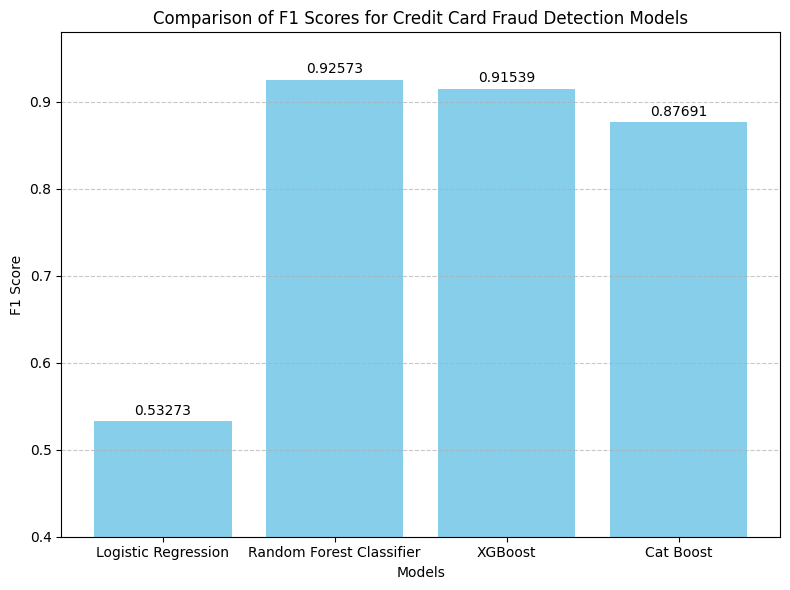
\includegraphics[scale=0.5]{figures/FinalPlot.png}
    \caption{Comparison of F1 Scores}
    \label{fig:Data Preprocessing}
\end{figure}
\clearpage


A bar plot visualization was utilized to compare the F1 scores, which indicates the Comparison of the F1 Scores of the four models. The graph showed that, in comparison to the other models, the Random Forest model performed the best and obtained the greatest F1 score.

This graphical representation made it very evident how much better the Random Forest model performed when detecting fraudulent transactions in the credit card system. These results demonstrate how important machine learning algorithms are in enhancing financial institutions' security against the constant danger of fraudulent activity. 


...





\section{Discussion and Analysis}

\subsection{Discussion}
The proposed project demonstrates the capabilities of machine learning algorithms in managing complex tasks such as adjusting to shifting fraud trends and unequal data distribution. The efficiency of the fraud detection system is verified by assessing model performance using measures like reliability, sensitivity, and precision. By using techniques like boosting using XGBoost and ensemble learning, the project can develop an in-depth knowledge of fraudulent actions, which enables preventative measures against new risks. 
The system demonstrates its adaptability in identifying fraudulent activity across various transaction patterns by mixing approaches such as Random Forest Classification, XGBoost, CatBoost, and Logistic Regression. Some significant discoveries and consequences from the project's outcomes are highlighted in the discussion of the credit card fraud detection system. First off, addressing the complicated challenges of fraud detection with a variety of machine learning techniques and deep learning models demonstrates an efficient plan of action.

\subsection{Summary}

Advanced fraud detection systems have been developed in response to the increasing susceptibility to credit card fraud caused by the fast growth of online transactions. The goal of this project is to build an efficient system for detecting credit card fraud by using deep learning models and machine learning methods. Results show how well the models work in detecting fraudulent activity, with the Random Forest model receiving the best F1 score out of all the methods evaluated. The use of performance measurements and visualization techniques highlights the critical function of machine learning algorithms in strengthening the security of financial transactions, providing financial institutions with powerful tools to successfully deal with  fraudulent activities. Using gathering and analyzing information from a Kaggle dataset, many supervised learning techniques—such as Random Forest Classification, XGBoost, CatBoost, and Logistic Regression—are implemented and optimized at the hyperparameter level. These models are trained with an extensive set of characteristics that include transaction details and past transactions to accurately distinguish between genuine and fraudulent transactions.

 






